\begin{figure}[h]
    \centering
    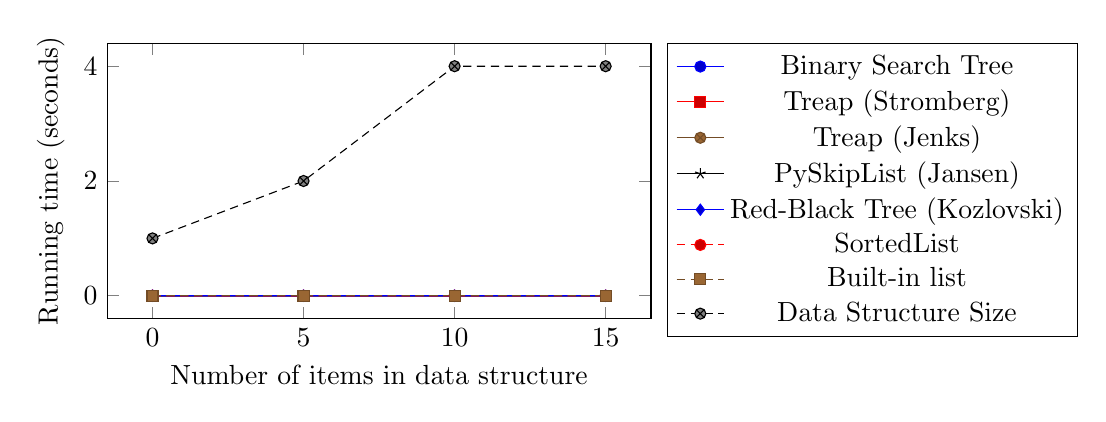
\begin{tikzpicture}
        \begin{axis}[
            xlabel={Number of items in data structure},
            ylabel={Running time (seconds)},
            title={},
            width=0.7\textwidth,
            height=2in,
            legend pos=outer north east
        ]
		\addplot coordinates {
			(0, 3.915279377771953e-06)
			(5, 3.212536925350946e-06)
			(10, 2.6101862518479687e-06)
			(15, 2.9113615885997465e-06)
		};
		\addplot coordinates {
			(0, 8.332517650129432e-06)
			(5, 6.525465629619633e-06)
			(10, 4.517630051275219e-06)
			(15, 3.7144958199373385e-06)
		};
		\addplot coordinates {
			(0, 6.826640966371411e-06)
			(5, 5.521547840447137e-06)
			(10, 5.320764282612811e-06)
			(15, 2.8109698096822947e-06)
		};
		\addplot coordinates {
			(0, 1.0842312123060237e-05)
			(5, 9.03526010255015e-06)
			(10, 7.830558755543617e-06)
			(15, 8.031342313377944e-06)
		};
		\addplot coordinates {
			(0, 1.3753673711659696e-05)
			(5, 9.135651881467312e-06)
			(10, 6.0235067350332405e-06)
			(15, 7.228208082040062e-06)
		};
		\addplot coordinates {
			(0, 4.51763005127493e-06)
			(5, 3.7144958199373385e-06)
			(10, 3.9152793777716644e-06)
			(15, 4.316846493440604e-06)
		};
		\addplot coordinates {
			(0, 1.4054849048411473e-06)
			(5, 1.5058766837585992e-06)
			(10, 1.4054849048411473e-06)
			(15, 1.5058766837585992e-06)
		};
		\addplot coordinates {
			(0, 1)
			(5, 2)
			(10, 4)
			(15, 4)
		};
        \legend{Binary Search Tree, Treap (Stromberg), Treap (Jenks), PySkipList (Jansen), Red-Black Tree (Kozlovski), SortedList, Built-in list, Data Structure Size}
        \end{axis}
    \end{tikzpicture}
    \caption{Average of 3 operations, benchmarked every 5, starting at 0.}
\end{figure}